\documentclass[thesis.tex]{subfiles}

\begin{document}

\chapter{Additional plots}

\begin{figure}
    \thisfloatpagestyle{empty}
    \makebox[\textwidth][c]{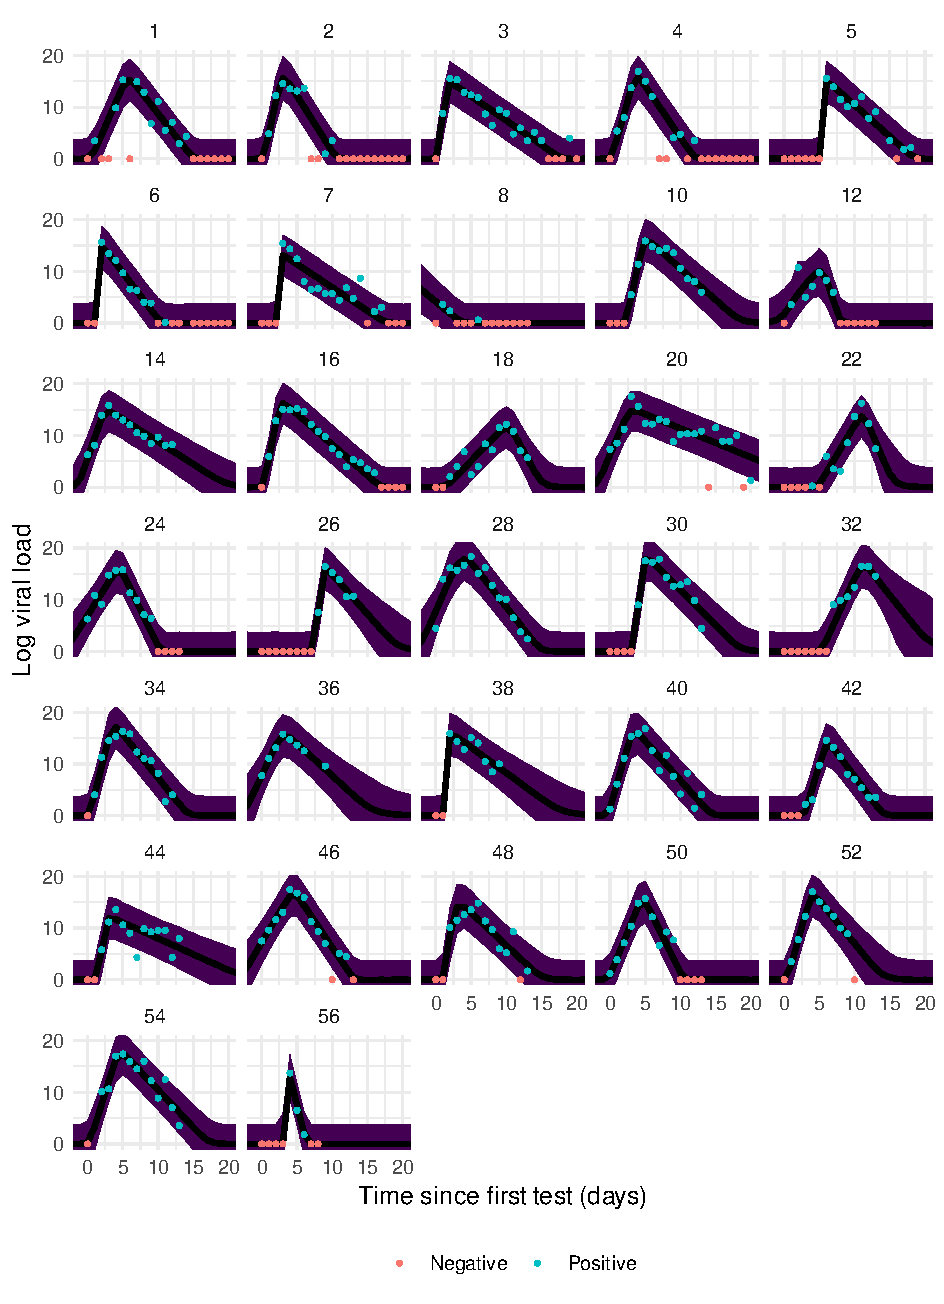
\includegraphics{ATACCC/appendix_fits}}
  \caption[Remaining ATACCC posterior predictive viral load fits]{
    Posterior predictive observed viral loads (median and 95\% CrI, lines and ribbon) from the model in \cref{E-ATACCC} for individuals not shown in \cref{E-ATACCC:fig:goodness-of-fits}, overlaid with their observed test results (dots). Posterior estimates are conditional on the result not being a false negative. Negative RT-PCR tests are plotted at the limit of detection, \ie a log viral load of 0. Each plot is labelled with the individual's position in the dataset, an arbitrary value.
  }
    \label{ATACCC:fig:appendix-goodness-of-fits}
\end{figure}

\begin{figure}
    \thisfloatpagestyle{empty}
    \makebox[\textwidth][c]{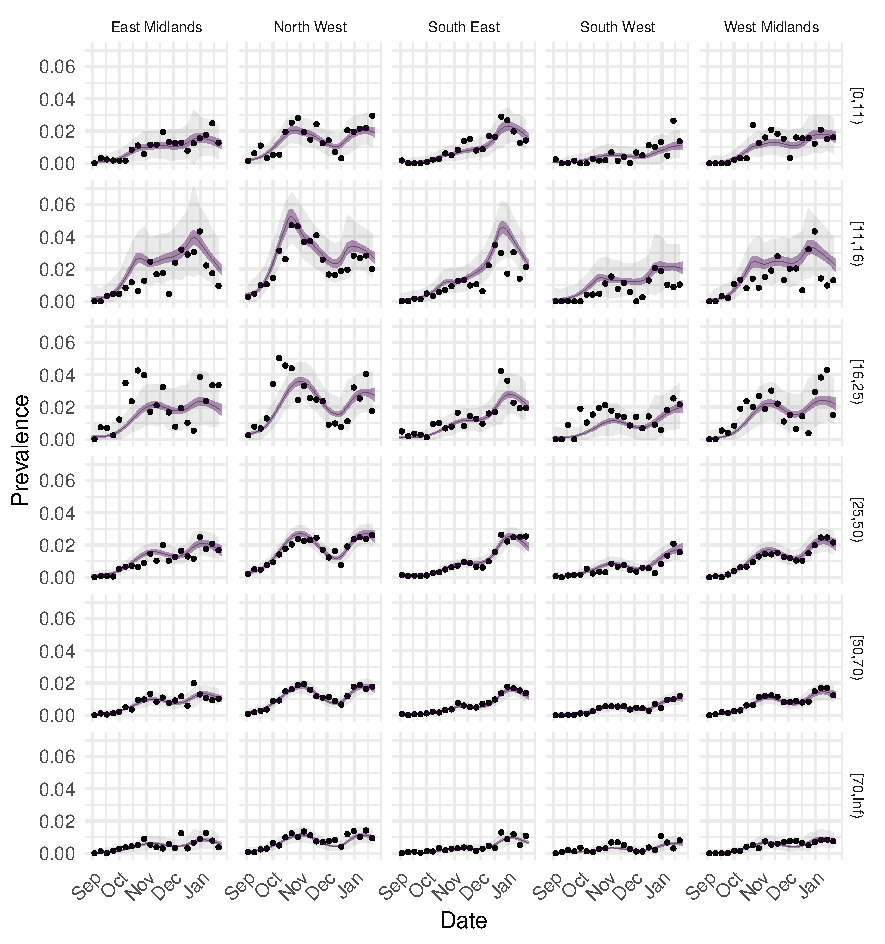
\includegraphics{SEIR/CIS/prev_appendix}}
    \captionsetup{width=0.8\paperwidth}
    \captionof{figure}[Other SEIR prevalence goodness-of-fit]{%
        Goodness-of-fit to prevalence data by region and age for selected regions (see \cref{SEIR:fig:prev} for others).
        The central ribbon and line show the posterior median and 95\% CrI estimate for the proportion of the relevant stratum RT-PCR positive on each day.
        The lighter outer ribbon is the 95\% posterior predictive interval for the proportion of test results that are positive each week.
        The dots show the observed prevalence in CIS, aggregated by week.
        For a well-calibrated model, 95\% of the dots would be within the outer ribbon.
    }
    \label{SEIR:fig:prev-appendix}
\end{figure}

\end{document}